% Options for packages loaded elsewhere
\PassOptionsToPackage{unicode}{hyperref}
\PassOptionsToPackage{hyphens}{url}
\PassOptionsToPackage{dvipsnames,svgnames,x11names}{xcolor}
%
\documentclass[
  article,
  nofooter]{jss}

\usepackage{amsmath,amssymb}
\usepackage{iftex}
\ifPDFTeX
  \usepackage[T1]{fontenc}
  \usepackage[utf8]{inputenc}
  \usepackage{textcomp} % provide euro and other symbols
\else % if luatex or xetex
  \usepackage{unicode-math}
  \defaultfontfeatures{Scale=MatchLowercase}
  \defaultfontfeatures[\rmfamily]{Ligatures=TeX,Scale=1}
\fi
\usepackage{lmodern}
\ifPDFTeX\else  
    % xetex/luatex font selection
\fi
% Use upquote if available, for straight quotes in verbatim environments
\IfFileExists{upquote.sty}{\usepackage{upquote}}{}
\IfFileExists{microtype.sty}{% use microtype if available
  \usepackage[]{microtype}
  \UseMicrotypeSet[protrusion]{basicmath} % disable protrusion for tt fonts
}{}
\makeatletter
\@ifundefined{KOMAClassName}{% if non-KOMA class
  \IfFileExists{parskip.sty}{%
    \usepackage{parskip}
  }{% else
    \setlength{\parindent}{0pt}
    \setlength{\parskip}{6pt plus 2pt minus 1pt}}
}{% if KOMA class
  \KOMAoptions{parskip=half}}
\makeatother
\usepackage{xcolor}
\setlength{\emergencystretch}{3em} % prevent overfull lines
\setcounter{secnumdepth}{-\maxdimen} % remove section numbering
% Make \paragraph and \subparagraph free-standing
\ifx\paragraph\undefined\else
  \let\oldparagraph\paragraph
  \renewcommand{\paragraph}[1]{\oldparagraph{#1}\mbox{}}
\fi
\ifx\subparagraph\undefined\else
  \let\oldsubparagraph\subparagraph
  \renewcommand{\subparagraph}[1]{\oldsubparagraph{#1}\mbox{}}
\fi


\providecommand{\tightlist}{%
  \setlength{\itemsep}{0pt}\setlength{\parskip}{0pt}}\usepackage{longtable,booktabs,array}
\usepackage{calc} % for calculating minipage widths
% Correct order of tables after \paragraph or \subparagraph
\usepackage{etoolbox}
\makeatletter
\patchcmd\longtable{\par}{\if@noskipsec\mbox{}\fi\par}{}{}
\makeatother
% Allow footnotes in longtable head/foot
\IfFileExists{footnotehyper.sty}{\usepackage{footnotehyper}}{\usepackage{footnote}}
\makesavenoteenv{longtable}
\usepackage{graphicx}
\makeatletter
\def\maxwidth{\ifdim\Gin@nat@width>\linewidth\linewidth\else\Gin@nat@width\fi}
\def\maxheight{\ifdim\Gin@nat@height>\textheight\textheight\else\Gin@nat@height\fi}
\makeatother
% Scale images if necessary, so that they will not overflow the page
% margins by default, and it is still possible to overwrite the defaults
% using explicit options in \includegraphics[width, height, ...]{}
\setkeys{Gin}{width=\maxwidth,height=\maxheight,keepaspectratio}
% Set default figure placement to htbp
\makeatletter
\def\fps@figure{htbp}
\makeatother

\usepackage{orcidlink,thumbpdf,lmodern}

\newcommand{\class}[1]{`\code{#1}'}
\newcommand{\fct}[1]{\code{#1()}}
\makeatletter
\@ifpackageloaded{caption}{}{\usepackage{caption}}
\AtBeginDocument{%
\ifdefined\contentsname
  \renewcommand*\contentsname{Table of contents}
\else
  \newcommand\contentsname{Table of contents}
\fi
\ifdefined\listfigurename
  \renewcommand*\listfigurename{List of Figures}
\else
  \newcommand\listfigurename{List of Figures}
\fi
\ifdefined\listtablename
  \renewcommand*\listtablename{List of Tables}
\else
  \newcommand\listtablename{List of Tables}
\fi
\ifdefined\figurename
  \renewcommand*\figurename{Figure}
\else
  \newcommand\figurename{Figure}
\fi
\ifdefined\tablename
  \renewcommand*\tablename{Table}
\else
  \newcommand\tablename{Table}
\fi
}
\@ifpackageloaded{float}{}{\usepackage{float}}
\floatstyle{ruled}
\@ifundefined{c@chapter}{\newfloat{codelisting}{h}{lop}}{\newfloat{codelisting}{h}{lop}[chapter]}
\floatname{codelisting}{Listing}
\newcommand*\listoflistings{\listof{codelisting}{List of Listings}}
\makeatother
\makeatletter
\makeatother
\makeatletter
\@ifpackageloaded{caption}{}{\usepackage{caption}}
\@ifpackageloaded{subcaption}{}{\usepackage{subcaption}}
\makeatother
\makeatletter
\@ifpackageloaded{tcolorbox}{}{\usepackage[skins,breakable]{tcolorbox}}
\makeatother
\makeatletter
\@ifundefined{shadecolor}{\definecolor{shadecolor}{rgb}{.97, .97, .97}}{}
\makeatother
\makeatletter
\makeatother
\makeatletter
\ifdefined\Shaded\renewenvironment{Shaded}{\begin{tcolorbox}[sharp corners, breakable, enhanced, boxrule=0pt, interior hidden, borderline west={3pt}{0pt}{shadecolor}, frame hidden]}{\end{tcolorbox}}\fi
\makeatother
\ifLuaTeX
  \usepackage{selnolig}  % disable illegal ligatures
\fi
\usepackage{bookmark}

\IfFileExists{xurl.sty}{\usepackage{xurl}}{} % add URL line breaks if available
\urlstyle{same} % disable monospaced font for URLs
\hypersetup{
  pdftitle={Why Americans Travel},
  pdfkeywords={key, words},
  colorlinks=true,
  linkcolor={blue},
  filecolor={Maroon},
  citecolor={Blue},
  urlcolor={Blue},
  pdfcreator={LaTeX via pandoc}}

%% -- Article metainformation (author, title, ...) -----------------------------

%% Author information
\author{Marion Bauman\\Georgetown University \And Aaron
Schwall\\Georgetown University \AND Varun Patel\\Georgetown
University \And Yuhan Cui\\Georgetown University}
\Plainauthor{Marion Bauman, Aaron Schwall, Varun Patel, Yuhan
Cui} %% comma-separated

\title{Why Americans Travel}
\Plaintitle{Why Americans Travel} %% without formatting

%% an abstract and keywords
\Abstract{INSERT ABSTRACT HERE}

%% at least one keyword must be supplied
\Keywords{key, words}
\Plainkeywords{key, words}

%% publication information
%% NOTE: Typically, this can be left commented and will be filled out by the technical editor
%% \Volume{50}
%% \Issue{9}
%% \Month{June}
%% \Year{2012}
%% \Submitdate{2012-06-04}
%% \Acceptdate{2012-06-04}
%% \setcounter{page}{1}
%% \Pages{1--xx}

%% The address of (at least) one author should be given
%% in the following format:
\Address{
Marion Bauman\\
Department of Data Science and Statistics\\
E-mail: \email{mfg77@georgetown.edu}\\
URL: \url{https://github.com/mfgeary}\\
\\~
Aaron Schwall\\
Department of Data Science and Statistics\\
\\~
Varun Patel\\
Department of Data Science and Statistics\\
\\~
Yuhan Cui\\
Department of Data Science and Statistics\\
\\~

}

\begin{document}
\maketitle

\section{Introduction}\label{introduction}

Americans are in constant transit, utilizing the national interstate and
highway system to travel various distances. Whether commuting to work,
taking vacations, visiting friends and family, transporting goods and
services, or engaging in commerce, people are constantly moving.
Understanding U.S. travel patterns provides essential insights into a
wide range of fields including environmental protection resource
allocation, urban planning, and economic trends. This research aims to
understand the motivation behind American travel based on trip
specifics. Specifically, we seek to predict the purpose of trips in
order to understand the connection between travel details and purpose
for travel.

\subsection{Relevant Research}\label{relevant-research}

A wide variety of industries and stakeholders are interested in
understanding travel habits and the usage of American transportation
networks.

\subsection{}\label{section}

\section{Methods}\label{methods}

\subsection{Data}\label{data}

As a federally funded agency, the Department of Transportation's Federal
Highway Administration seeks to understand how Americans are using the
national highway system. Since 1969, the FHA has regularly conducted the
National Highway Travel Survey (NHTS) in order to collect detailed data
on the travel habits of Americans and their usage of federal transit
networks \citep{userguide}. From January 2022 through January 2023, the
FHA conducted the 2022 NHTS, receiving responses from 7,XXX households
\citep{website}. Survey data includes in-depth information regarding
each household member's travel habits across the past 30 days, detailing
individual demographic information; household-level demographic
information; purpose, location, duration, and mode of transportation for
recent travel; and vehicle information \citep{datadictionary}.

For our research, we chose to utilize the individual demographic
information, called the \texttt{person} data, along with the trip
specific data, called the \texttt{trip} data. These two data sources
contained XX predictors that were unique for each observation. We
selected these table because 1) XX predictors was more than sufficient
for modeling, and 2) the household and vehicle level data was shared
across different observation, creating potential obfuscation in
modeling. The final joined data set of \texttt{person} and \texttt{trip}
data contained XXXX observations and XX features, including one target
variable.

\subsection{Preprocessing}\label{preprocessing}

To prepare the data for modeling, we conducting a thorough cleansing
process that included creating human-readable variable names and
removing missing or incomplete observations. The final data set was a
joined combination between person-level data and trip-level data. After
joining, all unique identifier variables and flag variables were removed
from the data.

Next, a correlation analysis was conducted to prevent autocorrelation or
multicollinearity between variables. An analysis revealed that three
variables had correlations over 0.2 with the target variable and were
highly related in content to the target variable. In order to build a
more robust model, these three variables, \texttt{why\_trip},
\texttt{trip\_purpose\_old\_schema}, and
\texttt{reason\_for\_travel\_to} were removed.

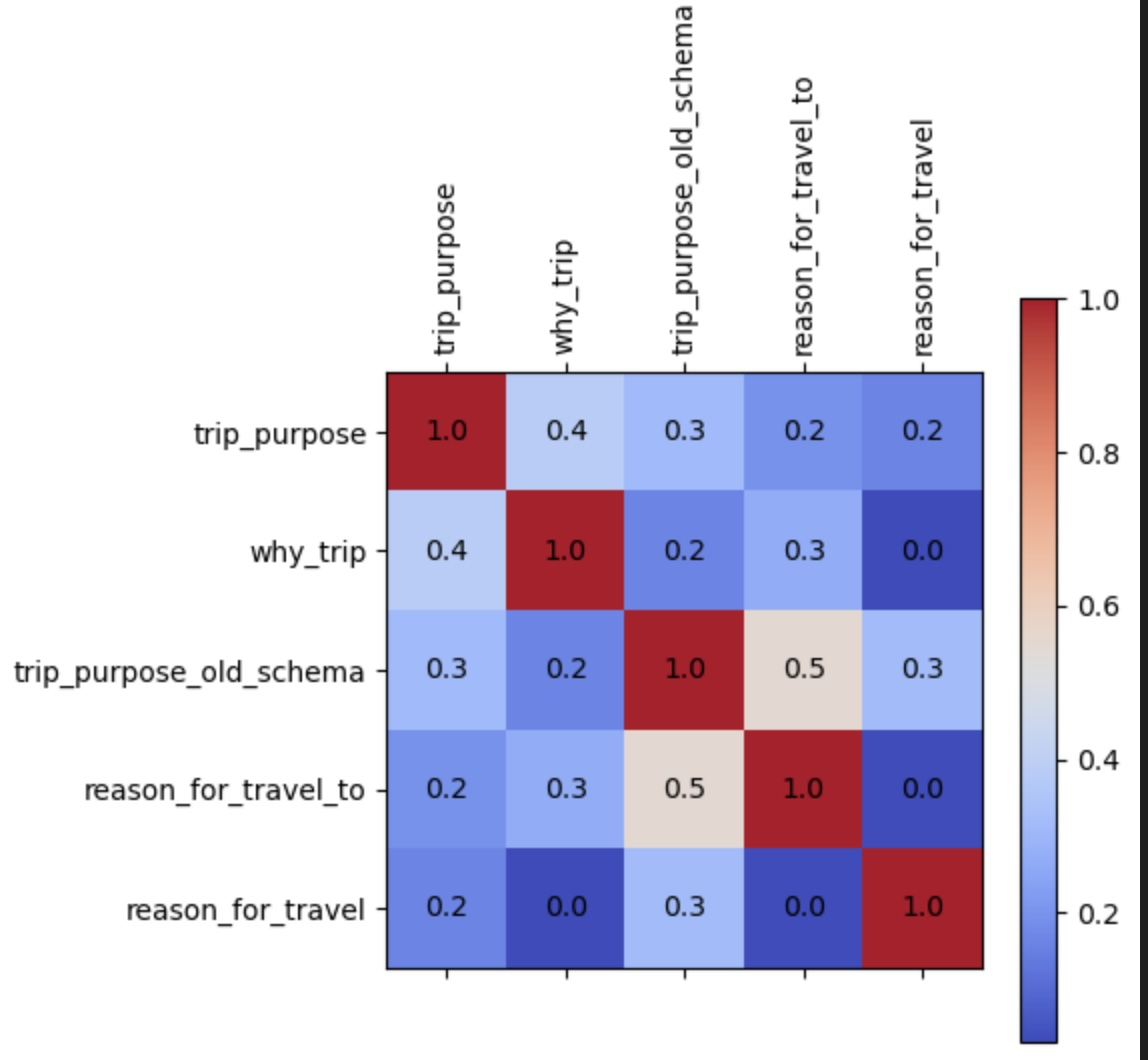
\includegraphics{imgs/correlation-matrix.jpg}

\section{Results}\label{results}

What are the results?

\section{Conclusion}\label{conclusion}

Conclusion here


  \bibliography{../code/poster/sources.bib}


\end{document}
